% !TEX root = ../../../main.tex

\toggletrue{image}
\toggletrue{imagehover}
\chapterimage{turtles}
\chapterimagetitle{\uppercase{TURTLES}}
\chapterimageurl{https://xkcd.com/889/}
\chapterimagehover{\small You're a turtle!}

\chapter{Mein erstes Programm}
\label{chapter-mein-erstes-programm}

Folgende Ziele erreichen Sie nach diesem Kapitel:

\newcommand{\meinErstesProgrammLernziele}{
\protect\begin{todolist}
\item Sie erklären, was eine \ac{IDE} ist und warum wir eine IDE einsetzen.
\item Sie erklären, was ein Ordner ist und erstellen auf Ihrem Computer einen Ordner.
\item Sie erklären, was eine Datei und eine Python-Datei ist.
\item Sie erstellen eine Python-Datei in einem vorgegebenen Ordner.
\end{todolist}
}

\lernziel{\autoref{chapter-mein-erstes-programm}, \nameref{chapter-mein-erstes-programm}}{\protect\meinErstesProgrammLernziele}

\meinErstesProgrammLernziele

\section{Quadrat zum Ersten}

\begin{example}

Unser erstes Python-Programm wird die Turtle dazu anweisen, ein Quadrat zu zeichnen. Mit diesem Programm können Sie gleichzeitig prüfen, ob die Installation der \ac{IDE} und Python geklappt hat. Erstellen Sie einen neuen Ordner mit dem Namen \graybgtexttt{01\_mein\_erstes\_programm}. Tippen Sie dann das \autoref{lst-quadrat} in eine \textbf{neue} Datei mit dem Namen  \graybgtexttt{quadrat.py} ab.


\begin{figure}[htb]
\centering
\begin{minipage}{0.55\linewidth}
\centering
\begin{lstlisting}[caption={Befehle für ein Quadrat (\graybgtexttt{quadrat.py}).}, label=lst-quadrat, showspaces=true]
import turtle

turtle.forward(100)
turtle.left(90)
turtle.forward(100)
turtle.left(90)
turtle.forward(100)
turtle.left(90)
turtle.forward(100)
turtle.left(90)
turtle.done()
\end{lstlisting}
\end{minipage}
\hfill
\begin{minipage}[c]{0.35\linewidth}
\centering
\begin{forest}
  pic dir tree,
  pic root,
  for tree={% folder icons by default; override using file for file icons
    directory,
  },
  [
  	imp\_prog
  	[
		00\_mein\_erstes\_programm
		[
			quadrat.py, pythonfile
		]	
    ]	
]
\end{forest}
\caption{Datei- und Ordnerstruktur in der \ac{IDE}.}
\label{figure-dir-structure-01}
\end{minipage}
\end{figure}

\begin{hinweis}
Das Zeichen \texttt{\char32} soll verdeutlichen, dass hier ein Leerzeichen\footnote{Leerschlag} eingegeben werden \textbf{muss}. Alle anderen Leerzeichen, welche nicht explizit abgedruckt sind, sollten aber müssen nicht notiert werden.
\end{hinweis}

Die Datei- und Ordnerstruktur sollte nun wie in \autoref{figure-dir-structure-01} aussehen. Führen Sie abschliessend das Programm aus. Wenn Sie das Programm ausführen, dann wird das Fenster aus \autoref{figure-quadrat} geöffnet und das Quadrat durch die \say{Turtle} (das kleine Dreieck) gezeichnet.

\begin{figure}[htb]
\centering
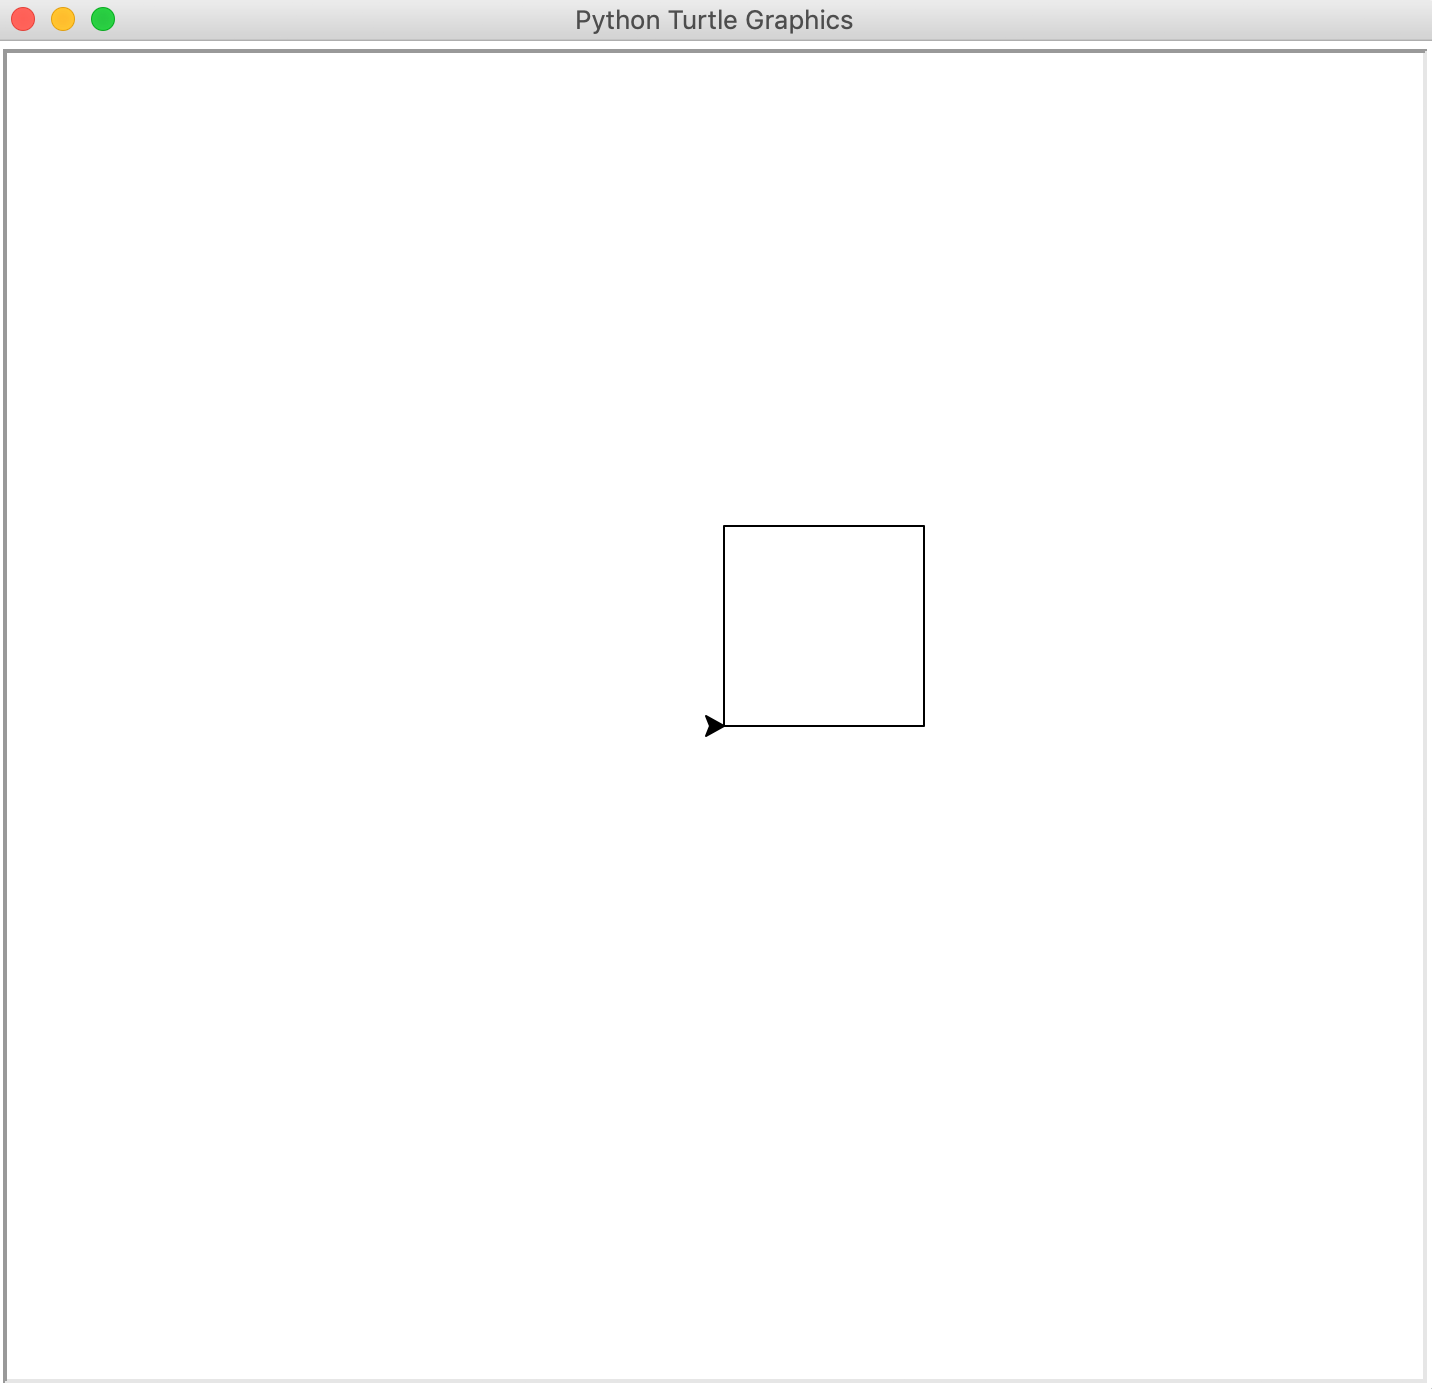
\includegraphics[scale=0.3]{quadrat.png}
\caption{Resultat der Ausführung unter macOS.}
\label{figure-quadrat}
\end{figure}

\end{example}

\section{Begriffe}

Wir klären hier zwei typische Begriffe aus dem Programmierumfeld.

\begin{definition}[Listing (dt.: Programmausdruck)]
Bezeichnung für den vollständigen Ausdruck des Source Codes eines Programms auf Papier. Listings dienen der Dokumentation eines Programms, der Fehlersuche (grösserer Überblick über das Programm als auf dem Bildschirm oder bei der Anzeige in einem Debugger) oder zu Lehrzwecken \cite{def-listing}.
\end{definition}

\begin{definition}[Source Code (dt.: Quellcode)]
Bezeichnung für den Programmtext, der ein Programmierer bzw. eine Programmiererin eingegeben hat. Wird oft einfach mit Code abgekürzt.
\end{definition}

\section{Zusammenfassung}

Typischerweise verwenden wir für das Erstellen eines Textes (z. B. einen Lebenslauf) ein Textverarbeitungsprogramm (z. B. Microsoft Word). Auch für das Programmieren ist es von Vorteil, wenn wir ein spezielles Programm verwenden. Solch ein Programm wird \textbf{\ac{IDE}} genannt. PyCharm ist zum Beispiel eine IDE und unterstützt uns beim Programmieren mit Python. Eine Software zu erstellen, wird häufig auch als Software-Entwicklung (engl. software development) bezeichnet. In einer \textbf{Datei} (engl. file) kann ein Computeranwender Informationen langfristig auf einem Speichermedium (Festplatte, USB-Stick, Cloud etc.) speichern. Die gespeicherten Informationen können sehr vielseitig sein: Texte, Bilder, Audio, \dots oder auch ein Python-Programm. Eine Datei, in der ein Python-Programm gespeichert ist, nennen wir \textbf{Python-Datei}. Eine Datei wird häufig unter Verwendung eines Punktes (\texttt{.}) in zwei Teile gegliedert, den eigentlichen Namen und die sogenannte \textbf{Dateinamen-Erweiterung} (engl. file extension). Für Word-Dateien gibt es zum Beispiel die Dateinamen-Erweiterung \texttt{.docx}. Python-Dateien haben die Dateinamen-Erweiterung \texttt{py}. In einem \textbf{Ordner} (engl. directory oder folder) können mehrere Dateien zusammengefasst werden. Ein Ordner kann wiederum auch einen weiteren Ordner besitzen.